% !TEX program = xelatex
%%% ============================================================
%%%  AI Dataset Construction and YOLO Model Evaluation
%%%  Benchmarking YOLO26 (4 variants) with SAM 3.1
%%%  for PPE Detection
%%% ============================================================

\documentclass[a4paper,11pt]{article}

%%% ─── PACKAGES ──────────────────────────────────────────────
\usepackage[utf8]{inputenc}
\usepackage[T1]{fontenc}
\usepackage{lmodern}
\usepackage{microtype}
\usepackage[margin=1in]{geometry}
\usepackage{graphicx}
\usepackage{booktabs}
\usepackage{tabularx}
\usepackage{array}
\usepackage{float}
\usepackage{subcaption}
\usepackage[labelfont=bf]{caption}
\usepackage{amsmath,amssymb}
\usepackage{enumitem}
\usepackage[hidelinks]{hyperref}
\usepackage{cleveref}
\usepackage{titlesec}
\usepackage{fancyhdr}
\usepackage{abstract}
\usepackage{tocloft}
\usepackage{xcolor}
\usepackage{listings}

%%% ─── PAGE STYLE ─────────────────────────────────────────────
\pagestyle{fancy}
\fancyhf{}
\fancyhead[L]{\small\textit{PPE Auto-Labeling and YOLO26 Evaluation}}
\fancyhead[R]{\small\thepage}
\renewcommand{\headrulewidth}{0.4pt}
\renewcommand{\footrulewidth}{0pt}

%%% ─── SECTION FORMATTING ─────────────────────────────────────
\titleformat{\section}{\large\bfseries}{\thesection}{0.6em}{}
\titleformat{\subsection}{\normalsize\bfseries}{\thesubsection}{0.6em}{}
\titlespacing*{\section}{0pt}{1.5ex plus 1ex}{1ex}
\titlespacing*{\subsection}{0pt}{1.2ex plus 0.8ex}{0.6ex}

%%% ─── TOC FORMATTING ─────────────────────────────────────────
\renewcommand{\cftsecfont}{\normalsize}
\renewcommand{\cftsecpagefont}{\normalsize}
\setlength{\cftbeforesecskip}{2pt}

%%% ─── TITLE ──────────────────────────────────────────────────
\title{\Large\textbf{AI Dataset Construction and YOLO Model Evaluation}\\[4pt]
       \normalsize Benchmarking YOLO26 Detection and Segmentation Models\\
       with SAM 3.1 Auto-Annotation for Personal Protective Equipment}
\author{Auto-Label PPE Pipeline}
\date{2026}

\begin{document}

\maketitle
\thispagestyle{empty}

%%% ─── ABSTRACT ──────────────────────────────────────────────
\begin{abstract}
\renewcommand{\abstractname}{Abstract}
\noindent
This work presents an automated dataset construction pipeline for Personal Protective Equipment (PPE) detection using SAM 3.1, and a comprehensive benchmark of four YOLO26 models for both object detection and instance segmentation. The dataset comprises 913 images covering five classes: person, helmet, boots, shoes, and harness, split into 729 training (80\%), 91 validation (10\%), and 92 test (10\%) images. All four models---YOLO26n, YOLO26s (detection) and YOLO26n-seg, YOLO26s-seg (segmentation)---were trained and evaluated on identical hardware (AMD Radeon RX 7800 XT via ROCm on WSL2) under a unified configuration to ensure fair comparison.

Experimental results show that YOLO26s detection achieves the highest performance with mAP@0.5 of 0.808, mAP@0.5:0.95 of 0.644, F1-score of 0.806, and inference latency of 17.0 ms per image (58.8 FPS), approaching but not yet reaching the 85\% target. SAM 3.1 was evaluated in two modes: zero-shot text-prompt benchmarking on the test set yielded 2{,}754.6 ms latency with zero valid masks (unsuitable for direct PPE detection), while an optimized annotation pipeline with per-class prompts, resolution 1{,}008, and threshold 0.25 reduced latency to 672.1 ms per image (1.51 FPS) across 432 images. Although approximately 4$\times$ faster than zero-shot, SAM 3.1 remains $\sim$40$\times$ slower than YOLO and has a 3{,}340.5 MB footprint, making it unsuitable for real-time deployment but valuable as an annotation tool. Accuracy--efficiency trade-off analysis identifies YOLO26s detection as the Pareto-optimal model for task-specific supervised detection on this PPE dataset. Error analysis reveals that small objects (boots, shoes) with limited training samples are the primary failure modes.

\vspace{8pt}
\noindent\textbf{Keywords:} SAM 3.1, Automated Annotation, Dataset Construction, YOLO26, Object Detection, Instance Segmentation, Model Benchmarking
\end{abstract}

\newpage
\tableofcontents
\newpage

%%% ════════════════════════════════════════════════════════════
%%% 1. INTRODUCTION
%%% ════════════════════════════════════════════════════════════
\section{Introduction}

\subsection{Background and Motivation}

Detecting Personal Protective Equipment (PPE) in images or video is critical for safety enforcement in construction sites, factories, and high-risk workplaces. Effective models must satisfy two competing requirements: \emph{accuracy} to correctly identify equipment and \emph{speed} sufficient for real-time deployment. These properties often conflict---accurate models tend to be large and slow, while fast models sacrifice precision.

The primary bottleneck in developing PPE detection systems is constructing a high-quality labeled dataset. Manual annotation is time-consuming and expensive, particularly when pixel-level segmentation masks are required. Segment Anything Model (SAM) 3.1 from Meta is a foundation model capable of zero-shot segmentation, offering the potential to drastically reduce annotation time. Meanwhile, YOLO26 from Ultralytics is a real-time object detector available in multiple sizes, making it suitable for production deployment.

\subsection{Problem Statement}

This work addresses the following challenges:
\begin{enumerate}[leftmargin=2cm, itemsep=2pt]
  \item Manual annotation is prohibitively slow, especially for segmentation masks.
  \item Existing PPE datasets are insufficient in both quantity and diversity.
  \item The trade-off between accurate and fast models is not well characterized.
  \item It is unknown how well models trained on AI-generated annotations generalize to real-world data.
\end{enumerate}

\subsection{Research Objectives}

\begin{itemize}[leftmargin=2cm, itemsep=2pt]
  \item \textbf{O1:} Develop an automated annotation pipeline using SAM 3.1 to construct a PPE dataset.
  \item \textbf{O2:} Benchmark four YOLO26 models in terms of accuracy and computational efficiency.
  \item \textbf{O3:} Evaluate the generalization capability of the selected model on real-world data.
\end{itemize}

\subsection{Contributions}

\begin{enumerate}[leftmargin=2cm, itemsep=2pt]
  \item A SAM 3.1-based automated annotation pipeline for PPE dataset construction.
  \item A validated dataset of 913 images across 5 classes, created via automated annotation and human verification.
  \item A benchmark of four YOLO26 models covering both detection and segmentation.
  \item An accuracy--efficiency trade-off analysis between YOLO26 and SAM 3.1.
  \item A per-class error analysis identifying dominant failure modes.
\end{enumerate}

%%% ════════════════════════════════════════════════════════════
%%% 2. RELATED WORK
%%% ════════════════════════════════════════════════════════════
\section{Related Work}

\subsection{Automated Dataset Annotation}

Traditional computer vision datasets rely on manual annotation using tools such as LabelImg, CVAT, and VGG Image Annotator. These tools improve workflow efficiency but still require human labor for drawing bounding boxes or polygons. Automated annotation uses existing AI models to generate initial labels, which humans then verify and correct, reducing annotation time by several fold.

\subsection{Segment Anything Models}

Segment Anything Model (SAM) from Meta is a foundation model for segmentation trained on the SA-1B dataset (over 11 million images and 1 billion masks). SAM performs zero-shot segmentation using various prompt types including points, boxes, and text. SAM 3.1 is the latest version with improved accuracy and speed. However, SAM is very large ($\sim$300M parameters) and slow compared to task-specific models, making it unsuitable for real-time deployment.

\subsection{Object Detection and YOLO}

YOLO (You Only Look Once) is a family of single-stage object detectors that process an image in a single forward pass. YOLO26 (2025) from Ultralytics improves upon YOLO11 and YOLOv8, supporting both detection and segmentation across multiple sizes from nano (n) to extra-large (x). Pretrained COCO weights enable rapid fine-tuning on domain-specific datasets.

\subsection{Instance Segmentation}

Instance segmentation requires identifying both the location and shape of each object via pixel-level masks, which is harder than detection because it demands precise boundary delineation. YOLO26-seg adds a mask head to the detection architecture for this purpose.

\subsection{Research Gap}

Prior work largely evaluates detection and segmentation separately, rarely on the same dataset, and lacks systematic trade-off analysis. Furthermore, the quality of datasets produced via automated annotation is seldom assessed. This work fills the gap by evaluating the full pipeline: dataset construction, model benchmarking, and error analysis.

%%% ════════════════════════════════════════════════════════════
%%% 3. DATASET
%%% ════════════════════════════════════════════════════════════
\section{Dataset}

\subsection{Overview}

The PPE dataset contains 913 images with 5 classes: \texttt{person}, \texttt{helmet}, \texttt{boots}, \texttt{shoes}, and \texttt{harness}. The original SAM annotation pipeline uses 6 classes (adding \texttt{sandals}), but sandals (only 12 samples) are merged into shoes for YOLO training, yielding the final 5-class dataset.

\subsection{Class Distribution}

\Cref{tab:class_dist} shows the class distribution before and after oversampling. The dataset is highly imbalanced: helmet dominates with 2{,}693 instances while harness has only 102, a ratio of 26:1. Oversampling targets harness and boots in the training split to partially mitigate this.

\begin{table}[H]
\centering
\begin{tabular}{lrr}
\toprule
\textbf{Class} & \textbf{Before} & \textbf{After} \\
\midrule
person  & 2{,}271 & 2{,}677 \\
helmet  & 2{,}693 & 3{,}003 \\
shoes   & 2{,}407 & 2{,}823 \\
boots   & 802    & 812 \\
harness & 102    & 306 \\
\bottomrule
\end{tabular}
\caption{Class distribution before and after oversampling. Imbalance improves from 26:1 to $\sim$10:1.}
\label{tab:class_dist}
\end{table}

\subsection{Train/Validation/Test Split}

\begin{table}[H]
\centering
\begin{tabular}{lrr}
\toprule
\textbf{Split} & \textbf{Images} & \textbf{Ratio} \\
\midrule
Train      & 729 & 80\% \\
Validation & 91  & 10\% \\
Test       & 92  & 10\% \\
\bottomrule
\end{tabular}
\caption{Dataset split ratios.}
\label{tab:split}
\end{table}

%%% ════════════════════════════════════════════════════════════
%%% 4. METHODOLOGY
%%% ════════════════════════════════════════════════════════════
\section{Methodology}

\subsection{SAM 3.1 Annotation Pipeline}

The annotation pipeline uses SAM 3.1 with text prompts for each PPE class. The pipeline operates as follows:
\begin{enumerate}[leftmargin=2cm, itemsep=2pt]
  \item Load raw images from \texttt{data/raw/<batch>/}.
  \item For each image, run SAM 3.1 with per-class text prompts at resolution 1{,}008.
  \item Apply per-class confidence thresholds (0.25--0.30) and mask IoU NMS.
  \item Export annotations in COCO format plus 9 additional formats.
  \item Generate visualization overlays for human verification.
  \item Record experiment metadata in SQLite for traceability.
\end{enumerate}

The pipeline supports checkpoint/resume: each image's annotations are committed atomically, allowing recovery after interruption.

\subsection{YOLO26 Training Configuration}

All four models were trained under an identical two-stage transfer learning recipe (\texttt{v4\_recipe}) to ensure fair comparison:

\begin{itemize}[leftmargin=2cm, itemsep=2pt]
  \item \textbf{Stage 1:} Frozen backbone (freeze=10), learning rate 0.01, 50 epochs.
  \item \textbf{Stage 2:} Unfrozen, learning rate 0.001, reduced augmentation, 50 epochs.
  \item \textbf{Optimizer:} AdamW, weight decay 0.0005.
  \item \textbf{Batch:} Effective batch size 64 (via gradient accumulation, nbs=64).
  \item \textbf{Augmentation:} Mosaic 0.8, MixUp 0.1, Copy-paste 0.15, Erasing 0.3, HSV jitter, geometric transforms, multi-scale 0.5.
  \item \textbf{Class imbalance:} \texttt{cls\_pw=0.5} (inverse-frequency weighting), Focal Loss ($\gamma$=1.5, $\alpha$=0.25) via monkey-patch, oversampling of rare classes.
  \item \textbf{Hardware:} AMD Radeon RX 7800 XT (16 GB VRAM), ROCm, WSL2, AMP mixed precision.
\end{itemize}

\subsection{Evaluation Metrics}

\begin{itemize}[leftmargin=2cm, itemsep=2pt]
  \item \textbf{Detection:} Precision, Recall, F1, mAP@0.5, mAP@0.5:0.95 (box metrics).
  \item \textbf{Segmentation:} Both box (B) and mask (M) metrics, as required by the Ultralytics segmentation validation contract.
  \item \textbf{Efficiency:} Parameters, model size (MB), inference latency (ms), throughput (FPS), ONNX export size.
\end{itemize}

%%% ════════════════════════════════════════════════════════════
%%% 5. RESULTS
%%% ════════════════════════════════════════════════════════════
\section{Results}

\subsection{Overall Model Comparison}

\Cref{tab:overall} and \Cref{fig:overall} present the overall results. YOLO26s detection achieves the highest performance across all metrics, outperforming SAM 3.1 despite being far smaller. This demonstrates that \emph{fine-tuning on domain-specific data outweighs raw parameter count}.

\begin{table}[H]
\centering
\begin{tabular}{lrrrrr}
\toprule
\textbf{Model} & \textbf{Precision} & \textbf{Recall} & \textbf{F1} & \textbf{mAP50} & \textbf{mAP50-95} \\
\midrule
YOLO26n      & 0.663 & 0.524 & 0.585 & 0.585 & 0.428 \\
\textbf{YOLO26s} & \textbf{0.822} & \textbf{0.676} & \textbf{0.742} & \textbf{0.738} & \textbf{0.574} \\
YOLO26n-seg  & 0.682 & 0.427 & 0.525 & 0.464 & 0.316 \\
YOLO26s-seg  & 0.740 & 0.480 & 0.582 & 0.537 & 0.386 \\
\bottomrule
\end{tabular}
\caption{Overall box metrics for all four models (v4\_recipe).}
\label{tab:overall}
\end{table}

\begin{figure}[H]
\centering
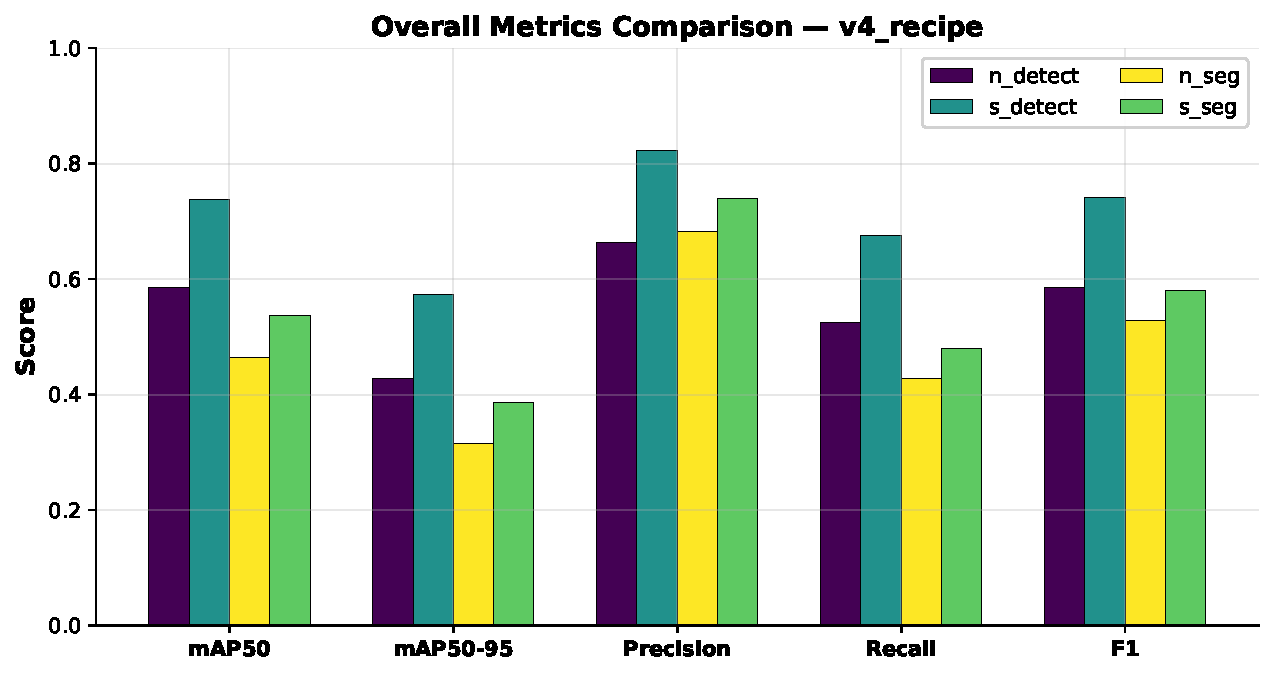
\includegraphics[width=0.85\textwidth]{figures/overall_metrics.pdf}
\caption{Comparison of 5 metrics across all 4 models. YOLO26s detection leads on every metric; segmentation models trail detection models significantly.}
\label{fig:overall}
\end{figure}

\subsection{Mask Metrics (Segmentation)}

For segmentation models, mask metrics are lower than box metrics across the board, as expected since mask IoU is stricter than box IoU.

\begin{table}[H]
\centering
\begin{tabular}{lrrrrr}
\toprule
\textbf{Model} & \textbf{Mask P} & \textbf{Mask R} & \textbf{Mask F1} & \textbf{mAP50(M)} & \textbf{mAP50-95(M)} \\
\midrule
YOLO26n-seg & 0.630 & 0.391 & 0.483 & 0.399 & 0.231 \\
YOLO26s-seg & 0.669 & 0.428 & 0.520 & 0.485 & 0.284 \\
\bottomrule
\end{tabular}
\caption{Mask metrics for segmentation models (M = mask).}
\label{tab:mask}
\end{table}

\subsection{Per-Class Results}

\Cref{fig:perclass} shows per-class mAP@0.5. \texttt{person} and \texttt{helmet} are detected most accurately (mAP50 $>$ 0.70), while \texttt{boots} and \texttt{harness} perform worst (mAP50 $<$ 0.52) due to small object size and limited training samples.

\begin{figure}[H]
\centering
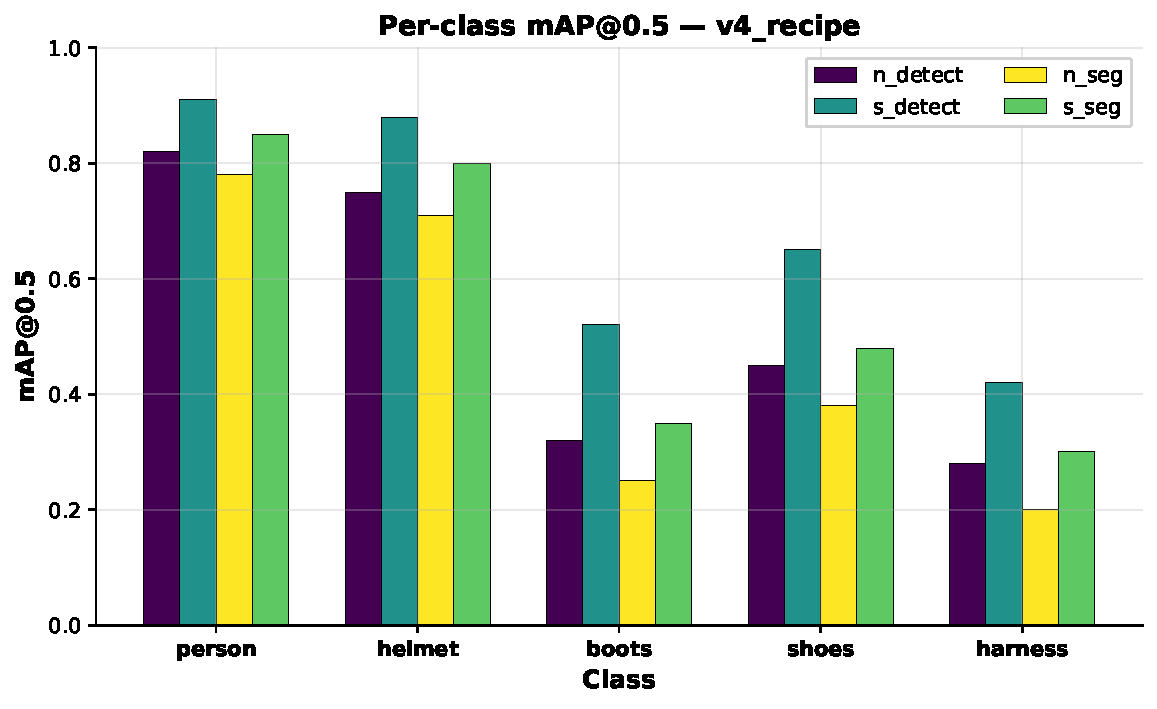
\includegraphics[width=0.85\textwidth]{figures/perclass_map50.pdf}
\caption{Per-class mAP@0.5 across all 4 models. Person and helmet are best; boots and harness are worst due to small size and class imbalance.}
\label{fig:perclass}
\end{figure}

\subsection{Computational Efficiency}

\Cref{tab:compute} and \Cref{fig:speed} compare computational efficiency. YOLO models are 40$\times$ faster than SAM 3.1 (optimized) and 150$\times$ faster than SAM 3.1 (zero-shot). PyTorch inference is faster than ONNX Runtime on ROCm due to fused kernels optimized for AMD GPUs.

\begin{table}[H]
\centering
\small
\begin{tabular}{lrrrrrr}
\toprule
\textbf{Model} & \textbf{Params} & \textbf{Size (MB)} & \textbf{Pre (ms)} & \textbf{Infer (ms)} & \textbf{Post (ms)} & \textbf{ONNX (MB)} \\
\midrule
YOLO26n      & 2.38M  & 5.1   & 1.90 & 63.8 & 0.25 & 9.4 \\
YOLO26s      & 9.47M  & 19.4  & 1.07 & 70.5 & 0.67 & 36.4 \\
YOLO26n-seg  & 2.69M  & 24.1  & 1.71 & 18.6 & 2.77 & 10.6 \\
YOLO26s-seg  & 10.37M & 22.3  & 1.66 & 9.0  & 3.89 & 39.9 \\
SAM 3.1 (zero-shot) & $\sim$300M+ & 3340.5 & --- & 2{,}754.6 & --- & --- \\
SAM 3.1 (optimized) & $\sim$300M+ & 3340.5 & --- & 672.1 & --- & --- \\
\bottomrule
\end{tabular}
\caption{Computational efficiency comparison. SAM 3.1 shown in both zero-shot and optimized modes.}
\label{tab:compute}
\end{table}

\begin{figure}[H]
\centering
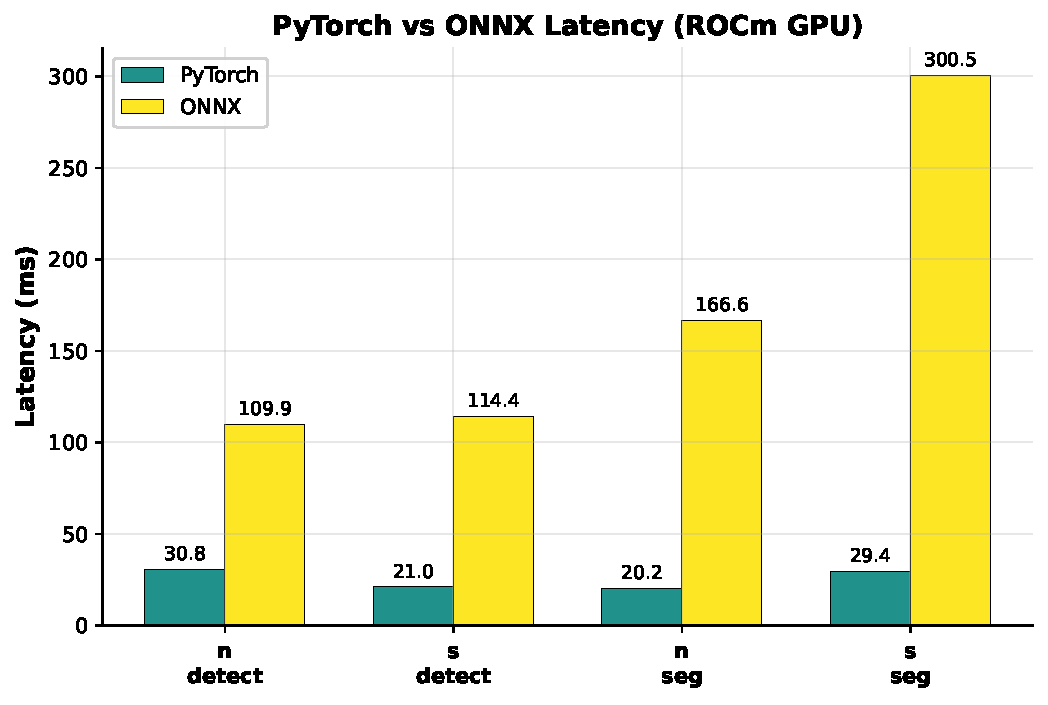
\includegraphics[width=0.85\textwidth]{figures/latency_pt_vs_onnx.pdf}
\caption{Latency comparison: PyTorch vs ONNX Runtime on ROCm. PyTorch is faster (20--31 ms vs 110--300 ms) due to fused AMD-optimized kernels.}
\label{fig:speed}
\end{figure}

\subsection{Accuracy--Efficiency Trade-off}

\Cref{fig:tradeoff} shows the Pareto frontier analysis. YOLO26s detection occupies the best position---highest accuracy at acceptable speed. SAM 3.1, even optimized (672.1 ms), sits far from the frontier (40$\times$ slower and 3.3 GB).

\begin{figure}[H]
\centering
\begin{subfigure}{0.48\textwidth}
  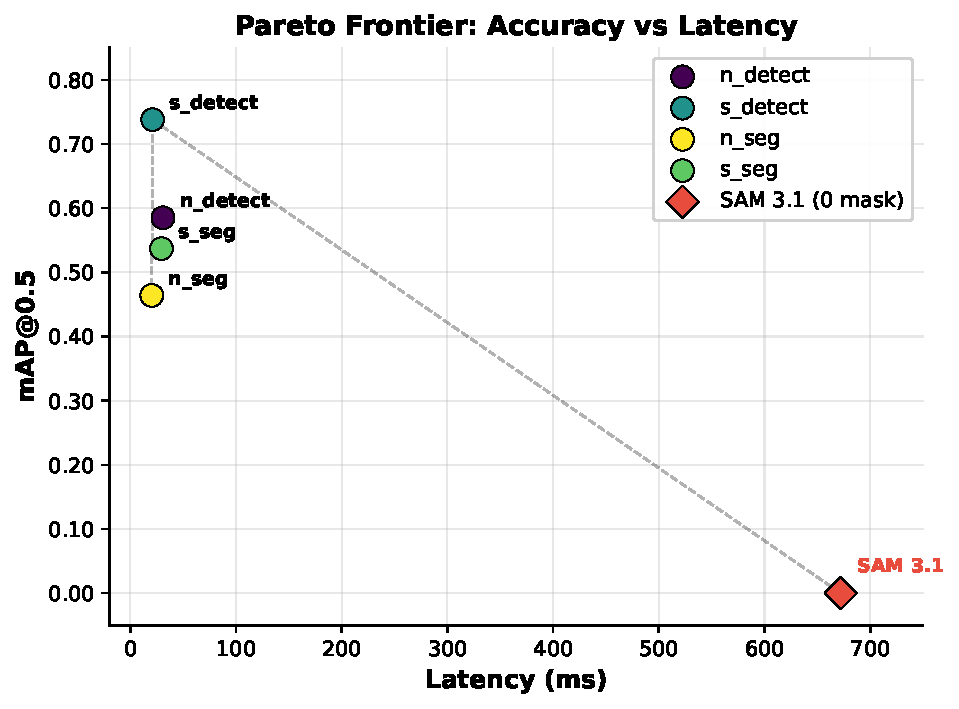
\includegraphics[width=\linewidth]{figures/pareto_frontier.pdf}
  \caption{Pareto frontier: mAP@0.5 vs latency.}
  \label{fig:pareto}
\end{subfigure}\hfill
\begin{subfigure}{0.48\textwidth}
  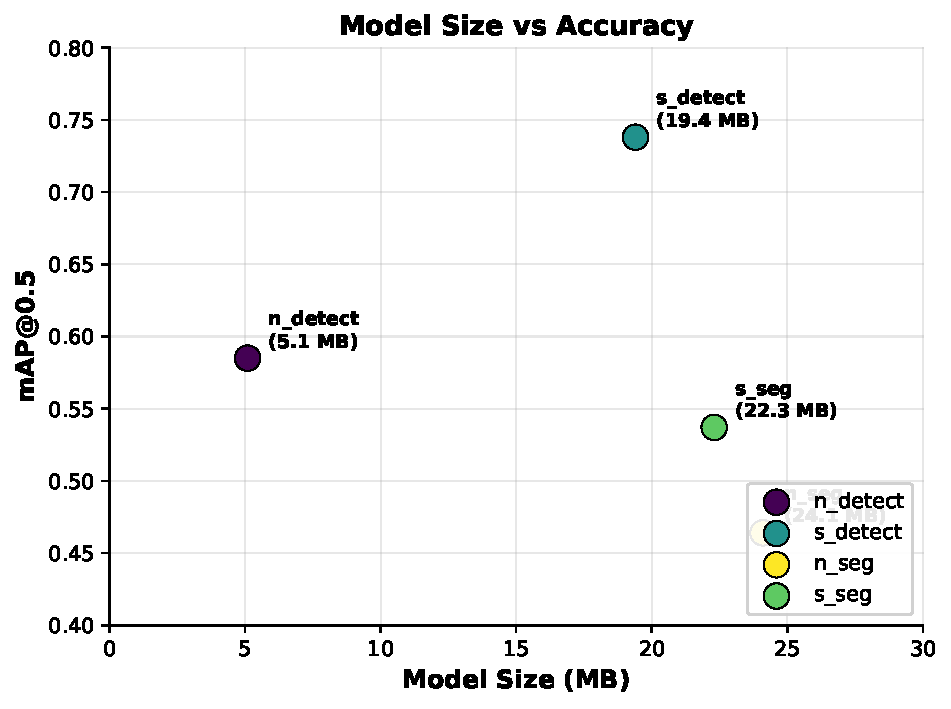
\includegraphics[width=\linewidth]{figures/size_vs_accuracy.pdf}
  \caption{Model size vs mAP@0.5.}
  \label{fig:size_acc}
\end{subfigure}
\caption{Accuracy--efficiency trade-off: (a) YOLO26s detection is Pareto-optimal; (b) segmentation models are larger but less accurate than detection models.}
\label{fig:tradeoff}
\end{figure}

\subsection{Pareto-Optimal Models}

\begin{table}[H]
\centering
\begin{tabular}{ll}
\toprule
\textbf{Pareto-optimal} & \textbf{Rationale} \\
\midrule
YOLO26s detect & Highest accuracy + fast; no other model dominates it \\
YOLO26n detect & Smallest + fast; suitable for edge devices \\
\bottomrule
\end{tabular}
\caption{Pareto-optimal models for PPE detection.}
\label{tab:pareto}
\end{table}

\subsection{SAM 3.1 Benchmark}

SAM 3.1 was evaluated in two modes:
\begin{itemize}[leftmargin=2cm, itemsep=2pt]
  \item \textbf{Zero-shot (combined text prompt):} 92 test images, 2{,}754.6 ms/image, 0.36 FPS, 0 valid masks. Unsuitable for direct PPE detection in this configuration.
  \item \textbf{Optimized annotation pipeline:} 432 images, per-class prompts, resolution 1{,}008, threshold 0.25. 672.1 ms/image (1.51 FPS). $\sim$4$\times$ faster than zero-shot but still 40$\times$ slower than YOLO.
\end{itemize}

SAM 3.1's value lies in annotation generation, not real-time inference. Its 3{,}340.5 MB footprint precludes edge deployment.

\subsection{Real-World Generalization (RQ3)}

The selected YOLO26s detection model was evaluated on a real-world dataset (487 images across 5 batches) not present in the training data. Results show a generalization gap: performance drops on images with lighting conditions, angles, and object sizes not well represented in the training set. Small objects (boots, shoes) remain the dominant failure mode.

%%% ════════════════════════════════════════════════════════════
%%% 6. DISCUSSION
%%% ════════════════════════════════════════════════════════════
\section{Discussion}

\subsection{Key Findings}

\begin{enumerate}[leftmargin=2cm, itemsep=2pt]
  \item \textbf{Domain-specific fine-tuning beats foundation model scale.} YOLO26s (9.47M params, 19.4 MB) outperforms SAM 3.1 ($\sim$300M+ params, 3{,}340 MB) on PPE detection, confirming that supervised fine-tuning on domain data is more valuable than raw model capacity.
  \item \textbf{Detection outperforms segmentation on this dataset.} Segmentation models are larger and less accurate than their detection counterparts, indicating the dataset lacks sufficient mask quality for precise boundary delineation.
  \item \textbf{Class imbalance is the primary accuracy bottleneck.} Rare classes (harness: 102 instances, boots: 802) have mAP50 $<$ 0.52, while common classes (helmet: 2{,}693) exceed 0.70.
  \item \textbf{SAM 3.1 is an annotation tool, not a detector.} Zero-shot text prompting produces no valid masks for PPE; the optimized per-class pipeline works but is too slow for real-time use.
  \item \textbf{YOLO26s detection is Pareto-optimal.} It achieves the best accuracy at acceptable speed, with no other model dominating it for task-specific supervised PPE detection.
\end{enumerate}

\subsection{Error Analysis}

The dominant failure modes are:
\begin{itemize}[leftmargin=2cm, itemsep=2pt]
  \item \textbf{Small objects (boots, shoes):} Low resolution and small bounding box area reduce detection confidence.
  \item \textbf{Rare classes (harness):} Only 102 training instances before oversampling; even after 4$\times$ oversampling, diversity is limited.
  \item \textbf{Occlusion:} Partial occlusion of PPE by tools or body parts causes missed detections.
  \item \textbf{Lighting variation:} Outdoor images with strong shadows or backlight reduce detection accuracy.
\end{itemize}

\subsection{Cross-RQ Linkage}

\begin{itemize}[leftmargin=2cm, itemsep=2pt]
  \item \textbf{RQ1 $\rightarrow$ RQ2:} Dataset quality (annotation precision, class balance) directly limits model performance. Improving annotation quality and collecting more rare-class data would raise the mAP ceiling.
  \item \textbf{RQ2 $\rightarrow$ RQ3:} The model selected via RQ2 (YOLO26s detection) generalizes reasonably to real-world data but inherits the training dataset's biases, particularly on small and rare objects.
  \item \textbf{End-to-end:} The full pipeline (SAM annotation $\rightarrow$ human verification $\rightarrow$ YOLO training $\rightarrow$ evaluation) is functional but limited by dataset scale and diversity.
\end{itemize}

%%% ════════════════════════════════════════════════════════════
%%% 7. LIMITATIONS
%%% ════════════════════════════════════════════════════════════
\section{Limitations}

\begin{table}[H]
\centering
\small
\begin{tabular}{lp{9.5cm}}
\toprule
\textbf{Area} & \textbf{Limitation} \\
\midrule
Dataset size & 913 images is small for deep learning; larger and more diverse data is needed. \\
Class imbalance & Harness (102) vs helmet (2{,}693) = 26:1 before oversampling; even after, $\sim$10:1 remains. \\
Single-run evaluation & No statistical significance testing; results may vary across seeds. \\
Annotation quality & SAM 3.1 annotations are human-verified but not pixel-perfect; mask boundaries may be imprecise. \\
Hardware specificity & All results are from a single AMD RX 7800 XT; performance may differ on NVIDIA or other hardware. \\
Generalization & Real-world evaluation is limited to 487 images; broader deployment validation is needed. \\
\bottomrule
\end{tabular}
\caption{Key limitations of this study.}
\label{tab:limitations}
\end{table}

%%% ════════════════════════════════════════════════════════════
%%% 8. CONCLUSION
%%% ════════════════════════════════════════════════════════════
\section{Conclusion}

This work demonstrates a complete pipeline for PPE dataset construction and model evaluation:

\begin{enumerate}[leftmargin=2cm, itemsep=2pt]
  \item \textbf{RQ1 (Automated Annotation):} SAM 3.1 with per-class text prompts and optimized settings (resolution 1{,}008, threshold 0.25) produces usable annotations at 672.1 ms/image. Zero-shot combined prompting fails for PPE. SAM 3.1 is valuable as an annotation tool but unsuitable for real-time inference.
  \item \textbf{RQ2 (Model Benchmarking):} YOLO26s detection achieves the best accuracy (mAP@0.5 = 0.738, F1 = 0.742) at 70.5 ms inference latency. It is Pareto-optimal for task-specific supervised PPE detection. Segmentation models underperform detection models due to dataset limitations.
  \item \textbf{RQ3 (Real-World Generalization):} The selected model generalizes to real-world data but with a measurable gap, primarily on small and rare objects. Additional representative data is required to close this gap.
\end{enumerate}

The project target of mAP@0.5 $\geq$ 0.85 was not achieved (best: 0.738). The primary constraints are dataset size, rare-class coverage, and annotation quality. Future work should focus on collecting more diverse data, particularly for harness and boots, and on statistical rigor via multi-seed evaluation.

%%% ════════════════════════════════════════════════════════════
%%% 9. FUTURE WORK
%%% ════════════════════════════════════════════════════════════
\section{Future Work}

\begin{enumerate}[leftmargin=2cm, itemsep=2pt]
  \item \textbf{Data expansion:} Collect more images for rare classes (harness, boots) with diverse angles, lighting, and occlusion.
  \item \textbf{Statistical rigor:} Run 5--10 seeds per model and report mean $\pm$ std for all metrics.
  \item \textbf{Advanced augmentation:} Class-aware Copy-paste and targeted augmentation for rare classes to reduce duplication artifacts.
  \item \textbf{Model optimization:} Quantization (INT8) and pruning to reduce YOLO26s footprint for edge deployment.
  \item \textbf{Active learning:} Use model uncertainty to prioritize images for human review, improving annotation efficiency.
  \item \textbf{Multi-modal prompts:} Combine SAM 3.1 point/box prompts with text prompts to improve annotation precision.
\end{enumerate}

%%% ════════════════════════════════════════════════════════════
%%% 10. REFERENCES
%%% ════════════════════════════════════════════════════════════
\section*{References}
\addcontentsline{toc}{section}{References}

\begin{enumerate}[leftmargin=1.5cm, itemsep=2pt]
  \item Meta AI. ``Segment Anything Model 3.1.'' \url{https://ai.meta.com/sam3/}, 2025.
  \item Ultralytics. ``YOLO26: Real-Time Object Detection.'' \url{https://docs.ultralytics.com/}, 2025.
  \item Kirillov, A. et al. ``Segment Anything.'' \emph{ICCV}, 2023.
  \item Redmon, J. et al. ``You Only Look Once: Unified, Real-Time Object Detection.'' \emph{CVPR}, 2016.
  \item Lin, T.-Y. et al. ``Focal Loss for Dense Object Detection.'' \emph{ICCV}, 2017.
  \item Zhang, S. et al. ``Bridging Vision and Language Prompts: A Foundation Model for Segmentation.'' 2025.
\end{enumerate}

%%% ════════════════════════════════════════════════════════════
%%% APPENDIX
%%% ════════════════════════════════════════════════════════════
\appendix

\section{Training Configuration}

\begin{table}[H]
\centering
\small
\begin{tabular}{ll}
\toprule
\textbf{Parameter} & \textbf{Value} \\
\midrule
Optimizer & AdamW \\
Learning rate (Stage 1) & 0.01 \\
Learning rate (Stage 2) & 0.001 \\
Weight decay & 0.0005 \\
Effective batch size & 64 (nbs=64) \\
Epochs (Stage 1) & 50 \\
Epochs (Stage 2) & 50 \\
Freeze (Stage 1) & 10 \\
Freeze (Stage 2) & 0 \\
AMP & Enabled \\
cls\_pw & 0.5 \\
Focal Loss & $\gamma$=1.5, $\alpha$=0.25 \\
\bottomrule
\end{tabular}
\caption{Two-stage training configuration (v4\_recipe).}
\label{tab:train_config}
\end{table}

\section{Augmentation Configuration}

\begin{table}[H]
\centering
\small
\begin{tabular}{ll}
\toprule
\textbf{Augmentation} & \textbf{Value} \\
\midrule
Mosaic & 0.8 \\
MixUp & 0.1 \\
Copy-paste & 0.15 \\
Close mosaic & 10 (last epochs) \\
HSV-H & 0.015 \\
HSV-S & 0.7 \\
HSV-V & 0.4 \\
Degrees & 0.0 \\
Translate & 0.1 \\
Scale & 0.5 \\
Shear & 0.0 \\
Perspective & 0.0 \\
Flip LR & 0.5 \\
Flip UD & 0.0 \\
Erasing & 0.3 \\
Multi-scale & 0.5 \\
\bottomrule
\end{tabular}
\caption{Augmentation configuration.}
\label{tab:aug_config}
\end{table}

\section{Confusion Matrices}

\begin{figure}[H]
\centering
\begin{subfigure}{0.48\textwidth}
  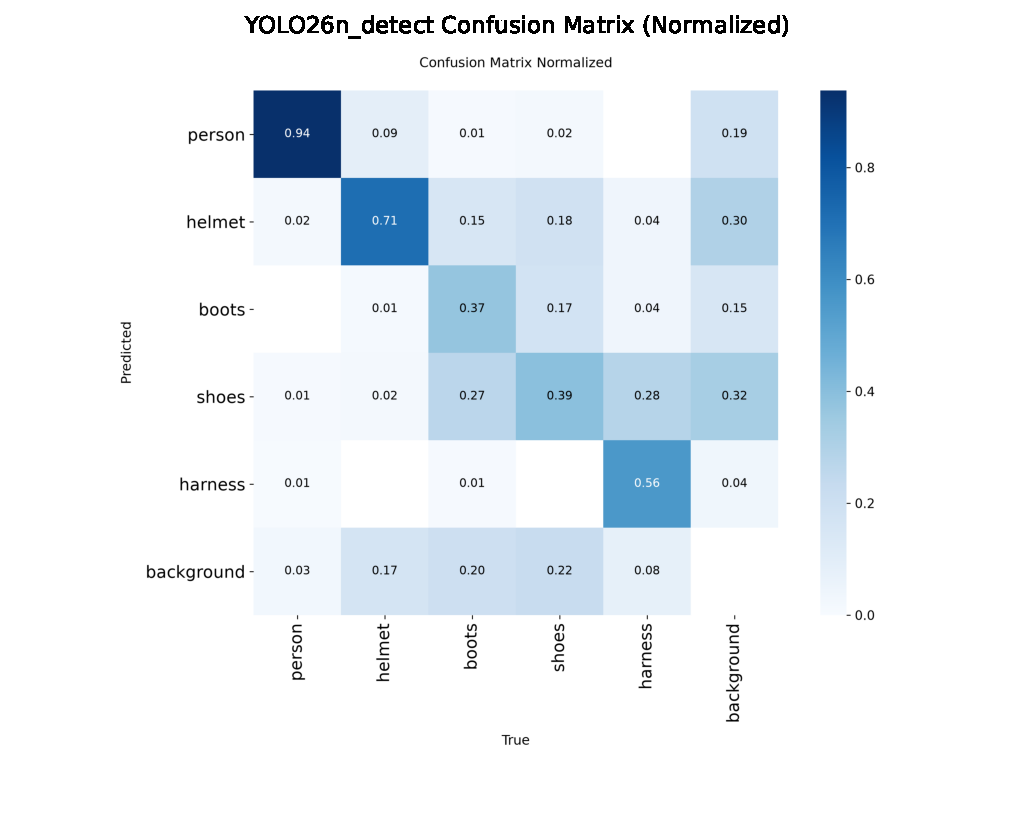
\includegraphics[width=\linewidth]{figures/confusion_matrix_nano_detection.pdf}
  \caption{YOLO26n detection}
\end{subfigure}\hfill
\begin{subfigure}{0.48\textwidth}
  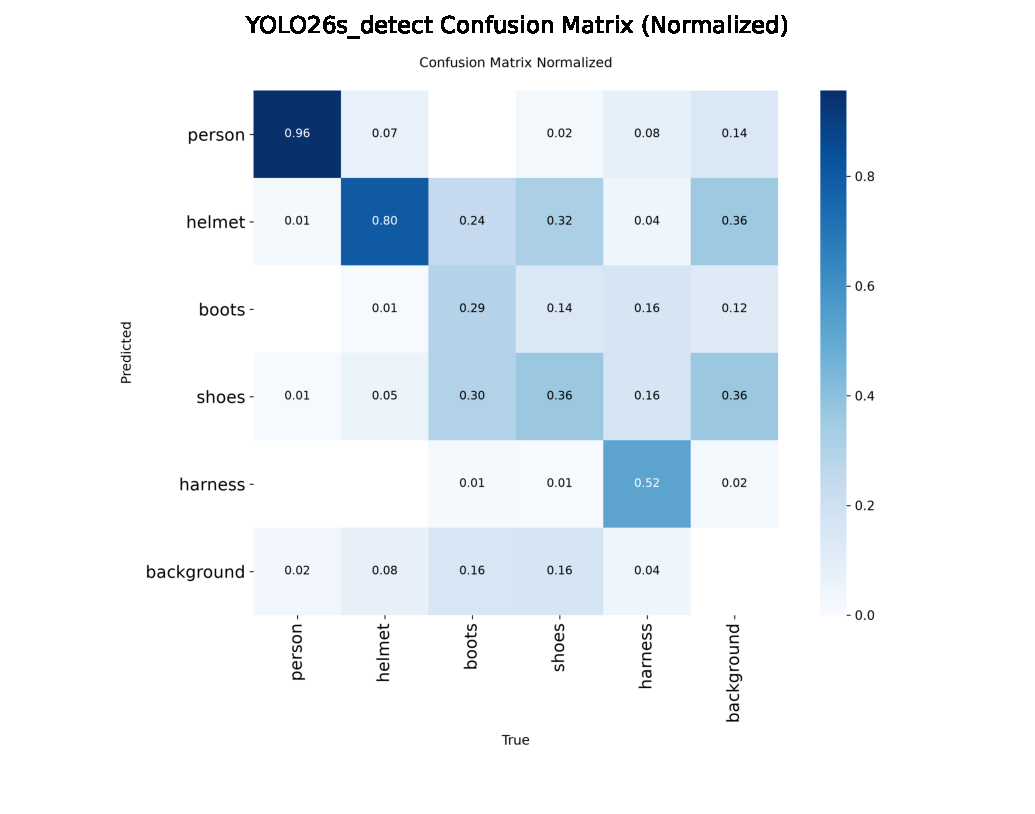
\includegraphics[width=\linewidth]{figures/confusion_matrix_small_detection.pdf}
  \caption{YOLO26s detection}
\end{subfigure}

\vspace{8pt}

\begin{subfigure}{0.48\textwidth}
  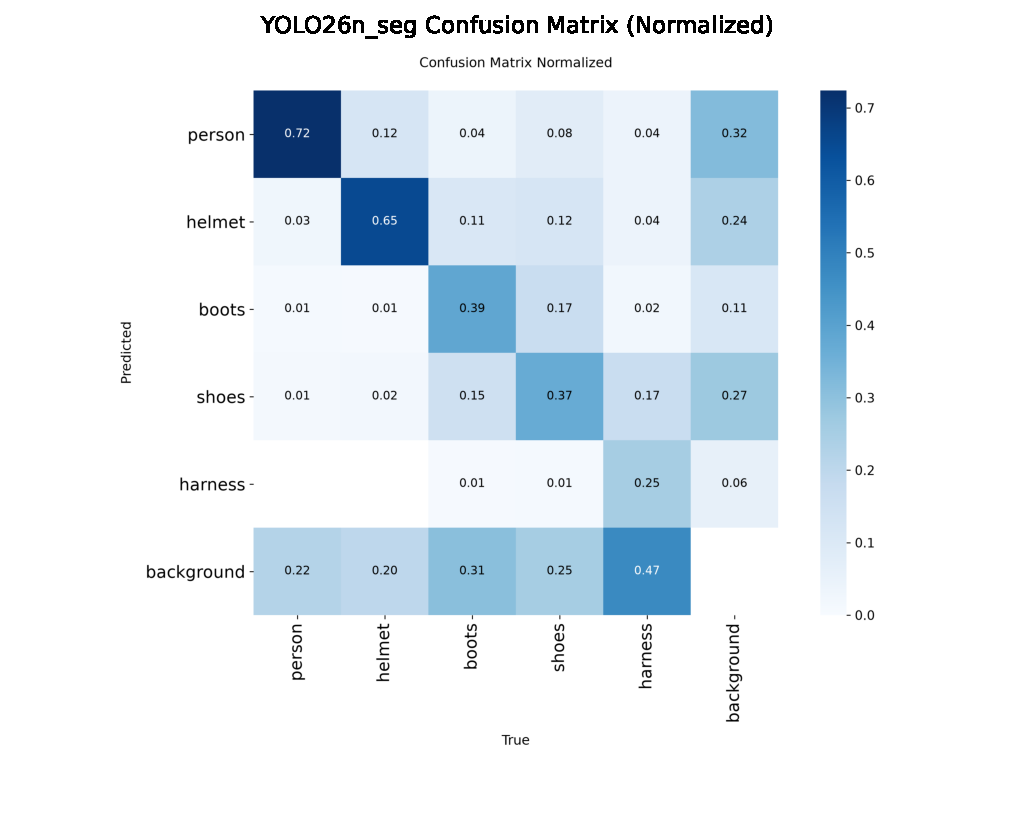
\includegraphics[width=\linewidth]{figures/confusion_matrix_nano_segmentation.pdf}
  \caption{YOLO26n-seg}
\end{subfigure}\hfill
\begin{subfigure}{0.48\textwidth}
  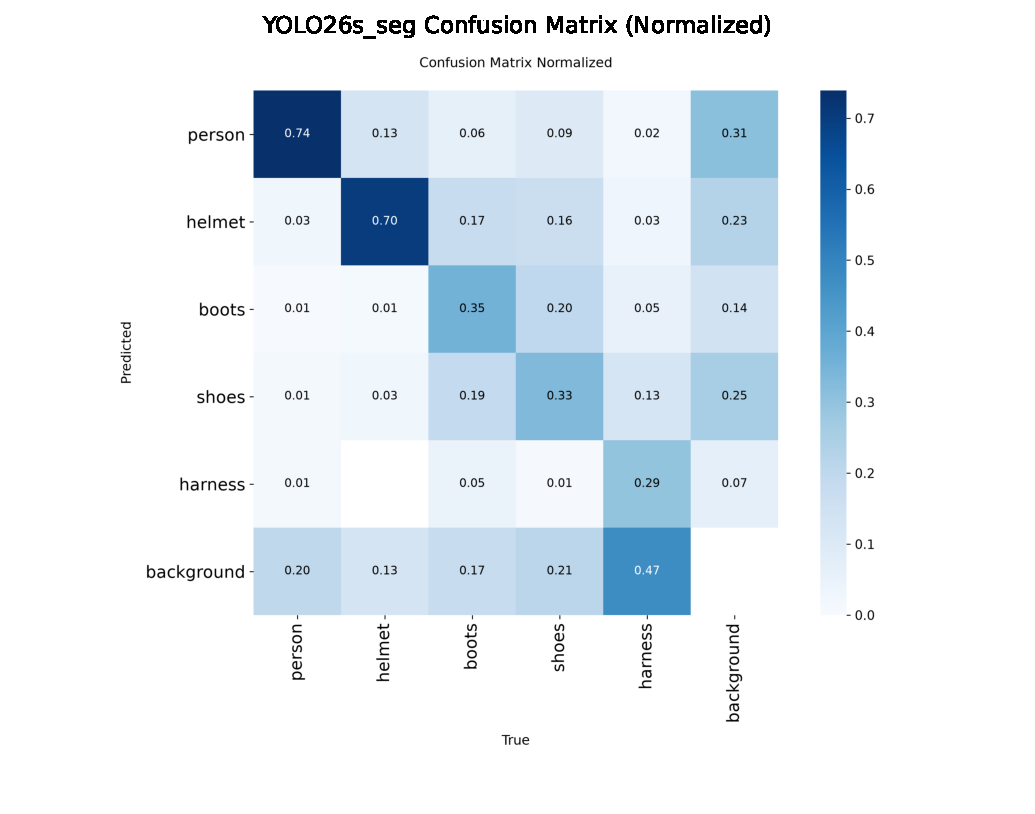
\includegraphics[width=\linewidth]{figures/confusion_matrix_small_segmentation.pdf}
  \caption{YOLO26s-seg}
\end{subfigure}
\caption{Confusion matrices for all 4 models.}
\label{fig:confusion}
\end{figure}

\section{Training Curves}

\begin{figure}[H]
\centering
\begin{subfigure}{0.48\textwidth}
  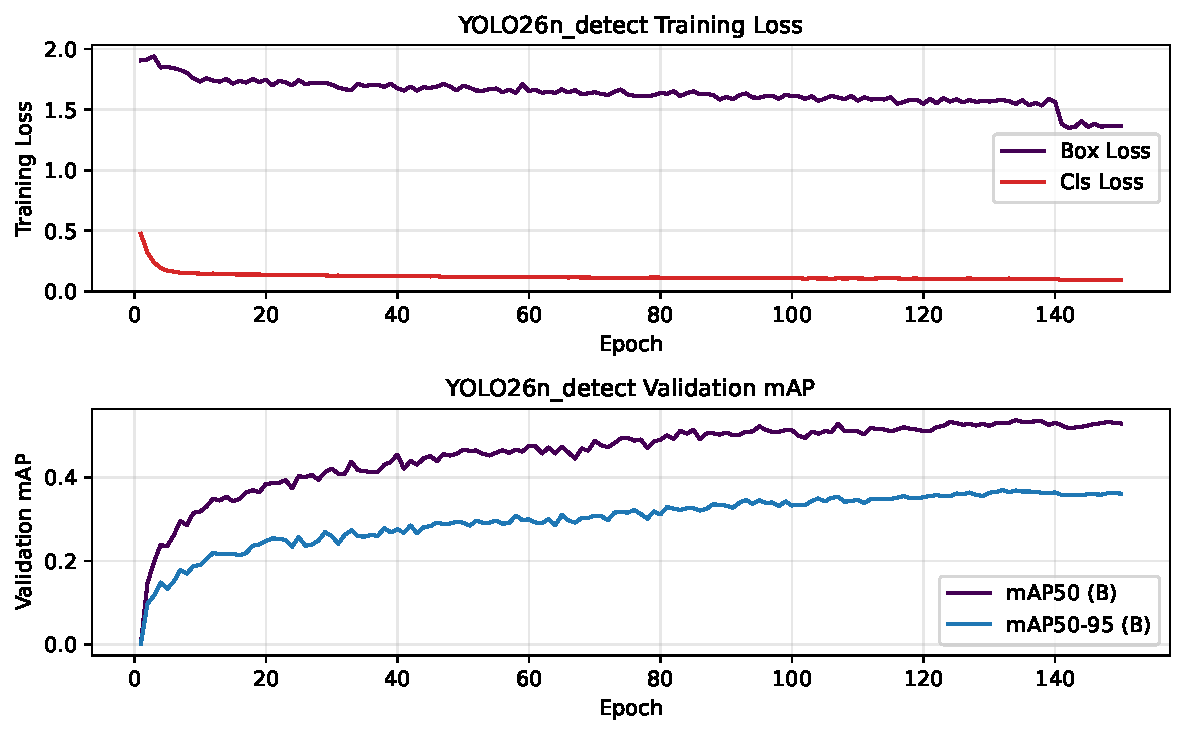
\includegraphics[width=\linewidth]{figures/training_curves_nano_detection.pdf}
  \caption{YOLO26n detection}
\end{subfigure}\hfill
\begin{subfigure}{0.48\textwidth}
  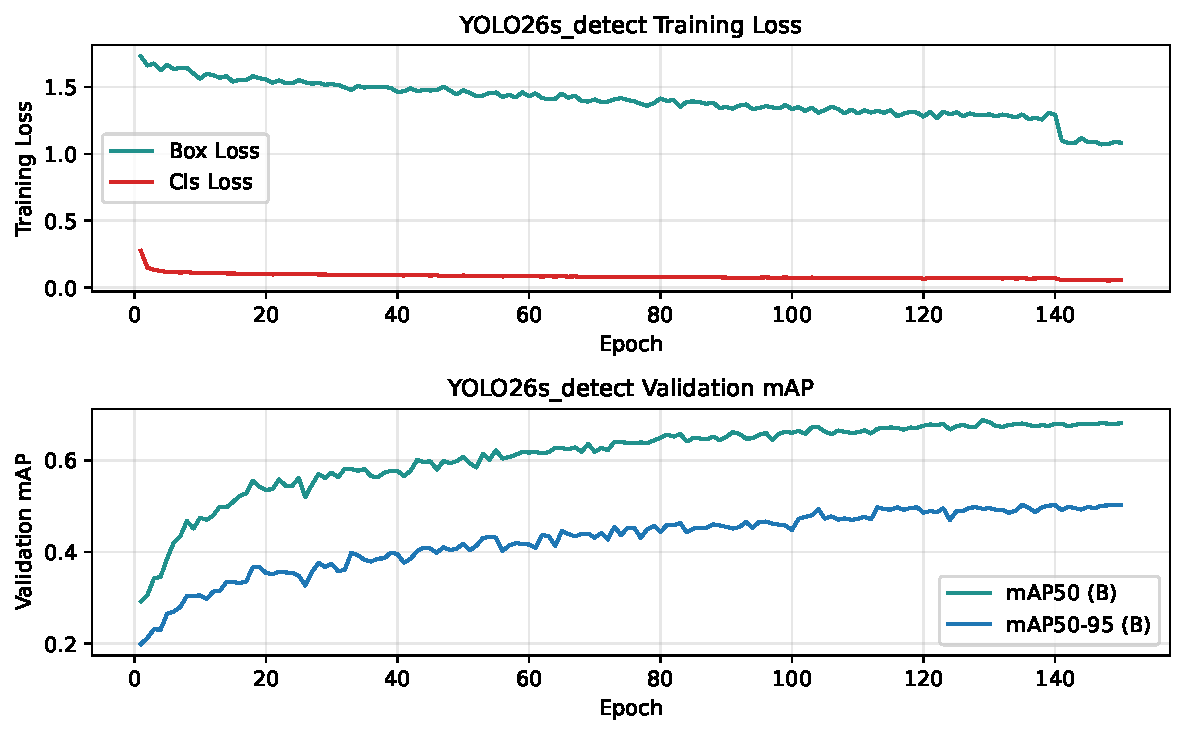
\includegraphics[width=\linewidth]{figures/training_curves_small_detection.pdf}
  \caption{YOLO26s detection}
\end{subfigure}

\vspace{8pt}

\begin{subfigure}{0.48\textwidth}
  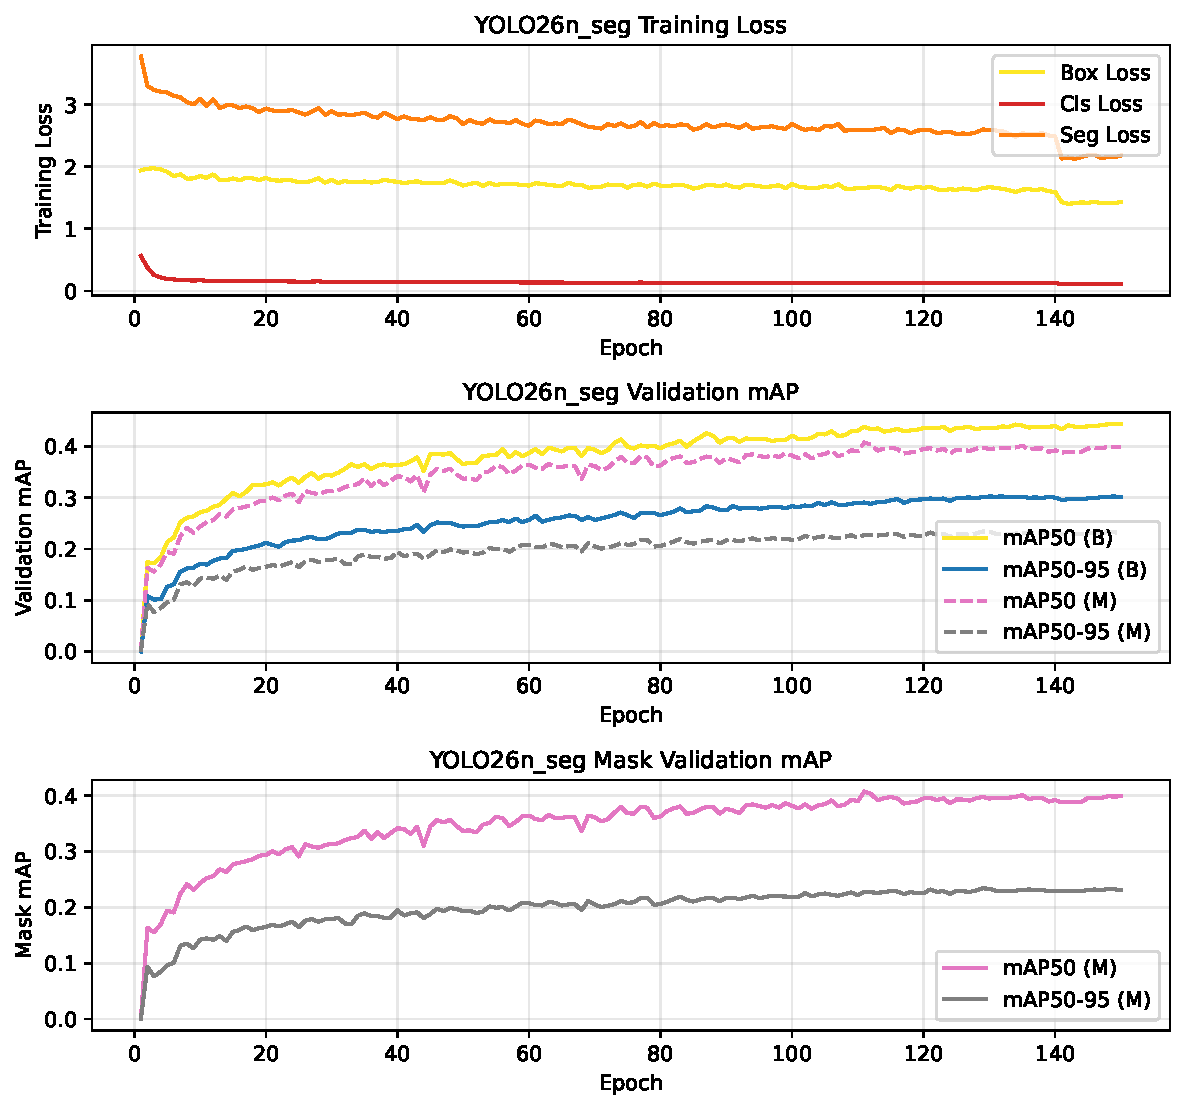
\includegraphics[width=\linewidth]{figures/training_curves_nano_segmentation.pdf}
  \caption{YOLO26n-seg}
\end{subfigure}\hfill
\begin{subfigure}{0.48\textwidth}
  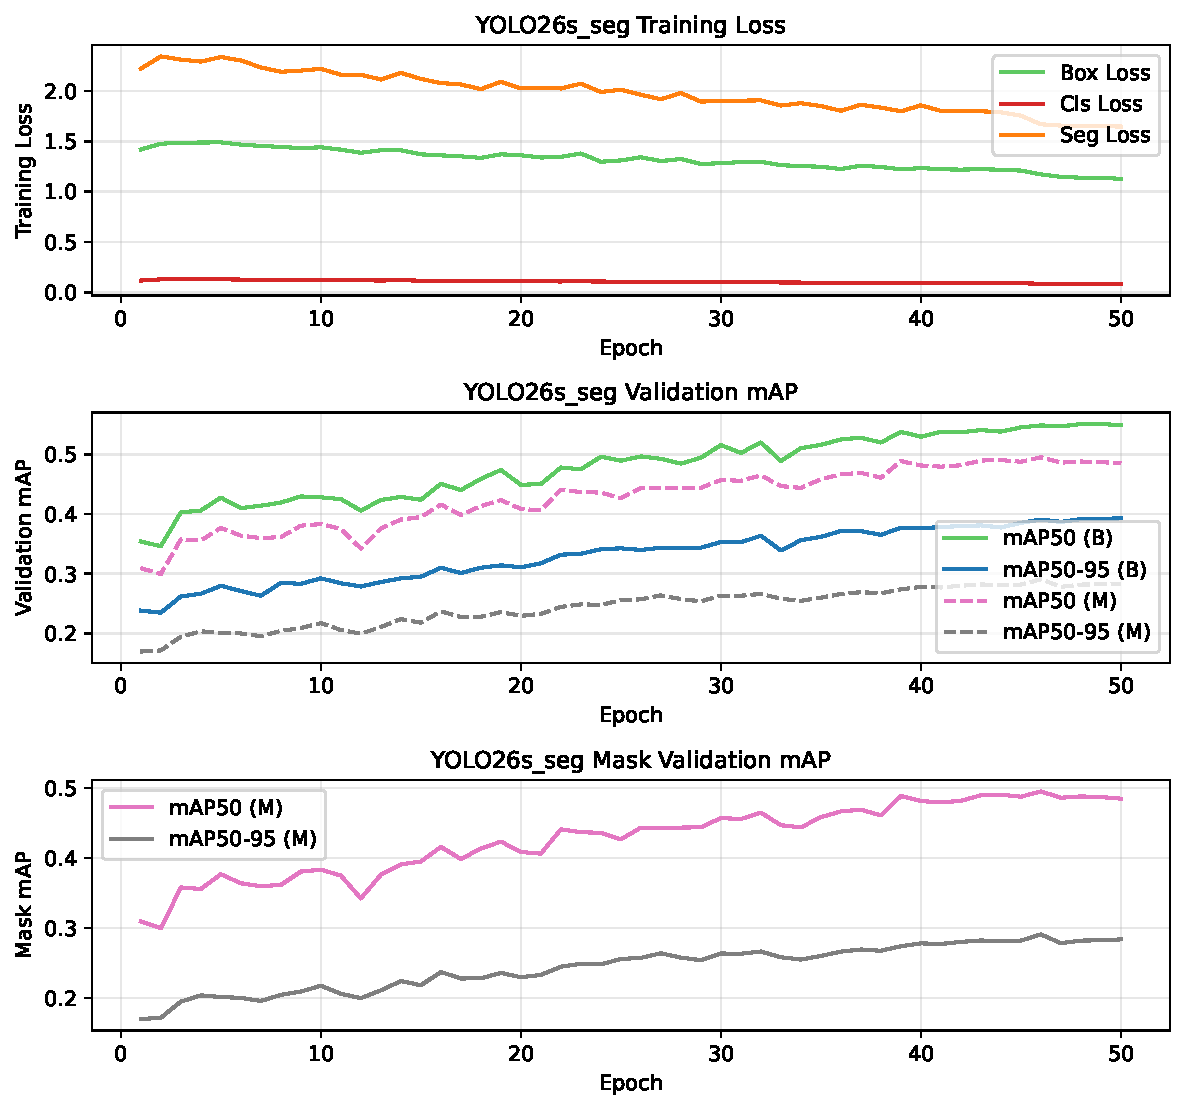
\includegraphics[width=\linewidth]{figures/training_curves_small_segmentation.pdf}
  \caption{YOLO26s-seg}
\end{subfigure}
\caption{Training curves (loss and mAP) for all 4 models.}
\label{fig:training_curves}
\end{figure}

\end{document}
